\documentclass[12pt,twoside]{article}
\usepackage[dvipsnames]{xcolor}
\usepackage{tikz,graphicx,amsmath,amsfonts,amscd,amssymb,bm,cite,epsfig,epsf,url}
\usepackage[hang,flushmargin]{footmisc}
\usepackage[colorlinks=true,urlcolor=blue,citecolor=blue]{hyperref}
\usepackage{amsthm,multirow,wasysym,appendix}
\usepackage{array,subcaption} 
% \usepackage[small,bf]{caption}
\usepackage{bbm}
\usepackage{pgfplots}
\usetikzlibrary{spy}
\usepgfplotslibrary{external}
\usepgfplotslibrary{fillbetween}
\usetikzlibrary{arrows,automata}
\usepackage{thmtools}
\usepackage{blkarray} 
\usepackage{textcomp}
\usepackage{pgf,tikz}
\usepackage{pgfplots}
\usepackage[left=0.8in,right=1.0in,top=1.0in,bottom=1.0in]{geometry}

%% Probability operators and functions
%
% \def \P{\mathrm{P}}
\def \P{\mathrm{P}}
\def \E{\mathrm{E}}
\def \Var{\mathrm{Var}}
\let\var\Var
\def \Cov {\mathrm{Cov}} \let\cov\Cov
\def \MSE {\mathrm{MSE}} \let\mse\MSE
\def \sgn {\mathrm{sgn}}
\def \R {\mathbb{R}}
\def \C {\mathbb{C}}
\def \N {\mathbb{N}}
\def \Z {\mathbb{Z}}
\def \cV {\mathcal{V}}
\def \cS {\mathcal{S}}

\newcommand{\RR}{\ensuremath{\mathbb{R}}}

\DeclareMathOperator*{\argmin}{arg\,min}
\DeclareMathOperator*{\argmax}{arg\,max}
\newcommand{\red}[1]{\textcolor{red}{#1}}
\newcommand{\blue}[1]{\textcolor{blue}{#1}}
\newcommand{\green}[1]{\textcolor{ForestGreen}{ #1}}
\newcommand{\fuchsia}[1]{\textcolor{RoyalPurple}{ #1}}



%
%% Probability distributions
%
%\def \Bern    {\mathrm{Bern}}
%\def \Binom   {\mathrm{Binom}}
%\def \Exp     {\mathrm{Exp}}
%\def \Geom    {\mathrm{Geom}}
% \def \Norm    {\mathcal{N}}
%\def \Poisson {\mathrm{Poisson}}
%\def \Unif    {\mathrm {U}}
%
\DeclareMathOperator{\Norm}{\mathcal{N}}

\newcommand{\bdb}[1]{\textcolor{red}{#1}}

\newcommand{\ml}[1]{\mathcal{ #1 } }
\newcommand{\wh}[1]{\widehat{ #1 } }
\newcommand{\wt}[1]{\widetilde{ #1 } }
\newcommand{\conj}[1]{\overline{ #1 } }
\newcommand{\rnd}[1]{\tilde{ #1 } }
\newcommand{\rv}[1]{ \rnd{ #1}  }
\newcommand{\rM}{\rnd{ m}  }
\newcommand{\rx}{\rnd{ x}  }
\newcommand{\ry}{\rnd{ y}  }
\newcommand{\rz}{\rnd{ z}  }
\newcommand{\ra}{\rnd{ a}  }
\newcommand{\rb}{\rnd{ b}  }
\newcommand{\rt}{\rnd{ t}  }
\newcommand{\rs}{\rnd{ s}  }


\newcommand{\rpc}{\widetilde{ pc}  }
\newcommand{\rndvec}[1]{\vec{\rnd{#1}}}

\def \cnd {\, | \,}
\def \Id { I }
\def \J {\mathbf{1}\mathbf{1}^T}

\newcommand{\op}[1]{\operatorname{#1}}
\newcommand{\setdef}[2]{ := \keys{ #1 \; | \; #2 } }
\newcommand{\set}[2]{ \keys{ #1 \; | \; #2 } }
\newcommand{\sign}[1]{\op{sign}\left( #1 \right) }
\newcommand{\trace}[1]{\op{tr}\left( #1 \right) }
\newcommand{\tr}[1]{\op{tr}\left( #1 \right) }
\newcommand{\inv}[1]{\left( #1 \right)^{-1} }
\newcommand{\abs}[1]{\left| #1 \right|}
\newcommand{\sabs}[1]{| #1 |}
\newcommand{\keys}[1]{\left\{ #1 \right\}}
\newcommand{\sqbr}[1]{\left[ #1 \right]}
\newcommand{\sbrac}[1]{ ( #1 ) }
\newcommand{\brac}[1]{\left( #1 \right) }
\newcommand{\bbrac}[1]{\big( #1 \big) }
\newcommand{\Bbrac}[1]{\Big( #1 \Big)}
\newcommand{\BBbrac}[1]{\BIG( #1 \Big)}
\newcommand{\MAT}[1]{\begin{bmatrix} #1 \end{bmatrix}}
\newcommand{\sMAT}[1]{\left(\begin{smallmatrix} #1 \end{smallmatrix}\right)}
\newcommand{\sMATn}[1]{\begin{smallmatrix} #1 \end{smallmatrix}}
\newcommand{\PROD}[2]{\left \langle #1, #2\right \rangle}
\newcommand{\PRODs}[2]{\langle #1, #2 \rangle}
\newcommand{\der}[2]{\frac{\text{d}#2}{\text{d}#1}}
\newcommand{\pder}[2]{\frac{\partial#2}{\partial#1}}
\newcommand{\derTwo}[2]{\frac{\text{d}^2#2}{\text{d}#1^2}}
\newcommand{\ceil}[1]{\lceil #1 \rceil}
\newcommand{\Imag}[1]{\op{Im}\brac{ #1 }}
\newcommand{\Real}[1]{\op{Re}\brac{ #1 }}
\newcommand{\norm}[1]{\left|\left| #1 \right|\right| }
\newcommand{\norms}[1]{ \| #1 \|  }
\newcommand{\normProd}[1]{\left|\left| #1 \right|\right| _{\PROD{\cdot}{\cdot}} }
\newcommand{\normTwo}[1]{\left|\left| #1 \right|\right| _{2} }
\newcommand{\normTwos}[1]{ \| #1  \| _{2} }
\newcommand{\normZero}[1]{\left|\left| #1 \right|\right| _{0} }
\newcommand{\normTV}[1]{\left|\left| #1 \right|\right|  _{ \op{TV}  } }% _{\op{c} \ell_1} }
\newcommand{\normOne}[1]{\left|\left| #1 \right|\right| _{1} }
\newcommand{\normOnes}[1]{\| #1 \| _{1} }
\newcommand{\normOneTwo}[1]{\left|\left| #1 \right|\right| _{1,2} }
\newcommand{\normF}[1]{\left|\left| #1 \right|\right| _{\op{F}} }
\newcommand{\normLTwo}[1]{\left|\left| #1 \right|\right| _{\ml{L}_2} }
\newcommand{\normNuc}[1]{\left|\left| #1 \right|\right| _{\ast} }
\newcommand{\normOp}[1]{\left|\left| #1 \right|\right|  }
\newcommand{\normInf}[1]{\left|\left| #1 \right|\right| _{\infty}  }
\newcommand{\proj}[1]{\mathcal{P}_{#1} \, }
\newcommand{\diff}[1]{ \, \text{d}#1 }
\newcommand{\vc}[1]{\boldsymbol{\vec{#1}}}
\newcommand{\rc}[1]{\boldsymbol{#1}}
\newcommand{\vx}{\vec{x}}
\newcommand{\vy}{\vec{y}}
\newcommand{\vz}{\vec{z}}
\newcommand{\vu}{\vec{u}}
\newcommand{\vv}{\vec{v}}
\newcommand{\vb}{\vec{\beta}}
\newcommand{\va}{\vec{\alpha}}
\newcommand{\vaa}{\vec{a}}
\newcommand{\vbb}{\vec{b}}
\newcommand{\vg}{\vec{g}}
\newcommand{\vw}{\vec{w}}
\newcommand{\vh}{\vec{h}}
\newcommand{\vbeta}{\vec{\beta}}
\newcommand{\valpha}{\vec{\alpha}}
\newcommand{\vgamma}{\vec{\gamma}}
\newcommand{\veta}{\vec{\eta}}
\newcommand{\vnu}{\vec{\nu}}
\newcommand{\rw}{\rnd{w}}
\newcommand{\rvnu}{\vc{\nu}}
\newcommand{\rvv}{\rndvec{v}}
\newcommand{\rvw}{\rndvec{w}}
\newcommand{\rvx}{\rndvec{x}}
\newcommand{\rvy}{\rndvec{y}}
\newcommand{\rvz}{\rndvec{z}}
\newcommand{\rvX}{\rndvec{X}}


\newtheorem{theorem}{Theorem}[section]
% \declaretheorem[style=plain,qed=$\square$]{theorem}
\newtheorem{corollary}[theorem]{Corollary}
\newtheorem{definition}[theorem]{Definition}
\newtheorem{lemma}[theorem]{Lemma}
\newtheorem{remark}[theorem]{Remark}
\newtheorem{algorithm}[theorem]{Algorithm}

% \theoremstyle{definition}
%\newtheorem{example}[proof]{Example}
\declaretheorem[style=definition,qed=$\triangle$,sibling=definition]{example}
\declaretheorem[style=definition,qed=$\bigcirc$,sibling=definition]{application}

%
%% Typographic tweaks and miscellaneous
%\newcommand{\sfrac}[2]{\mbox{\small$\displaystyle\frac{#1}{#2}$}}
%\newcommand{\suchthat}{\kern0.1em{:}\kern0.3em}
%\newcommand{\qqquad}{\kern3em}
%\newcommand{\cond}{\,|\,}
%\def\Matlab{\textsc{Matlab}}
%\newcommand{\displayskip}[1]{\abovedisplayskip #1\belowdisplayskip #1}
%\newcommand{\term}[1]{\emph{#1}}
%\renewcommand{\implies}{\;\Rightarrow\;}



\begin{document}

\begin{center}
{\large{\textbf{Homework 0}} } \vspace{0.2cm}\\
Due September 12 at 11 pm
\\
\end{center}
Name: Giulio Duregon

\begin{enumerate}

\item (Sets) We will use set theory to define probability spaces. Are these statements true or false? Provide a proof if they are true (you can use Venn diagrams to gain intuition, but also write down a formal proof), or a counterexample if they are false. 
\begin{enumerate}
\item[] A partition of a set $\Omega$ is a collection of sets $S_1$, \ldots, $S_n$ such that $\Omega = \cup_{i}S_i$ and $S_i \cap S_j = \emptyset$ for $i\neq j$. 
\item If  $S_1$, \ldots, $S_n$ is a partition of $\Omega$, then for any subset $A \subseteq \Omega$, $S_1 \cap A$, \ldots, $S_n \cap A$ is a partition of $A$.
\subitem
This statement is true, as $A = \cup_{i}S_i \cap A$ (I'm not sure if I wrote this correctly mathematically, but what I'm trying to say is that if we add (by taking the union) all the intersections between $A$ and $S_1, \dots, S_n$ they will add up to A).\par
Also,  $(A \cap S_i) \cap (A \cap S_j) = \emptyset$ for $i\neq j$ (Again, not sure if I wrote this correctly, but what I am trying to express is that since $S_1, \dots, S_n$ is a partition of $\Omega$ by definition it is disjoint, so every $A\cap S_i$ will be disjoint from every other $A\cap S_j$ where $i\neq j$).

\item For any sets $A$ and $B$, $A^c \cup B^c = (A \cup B)^c$. 
\subitem This statement is false, which will be proven by counter example. Consider the sample space where $A,B \in \Omega$ and $A \cap B \neq \emptyset$ (I am trying to describe the classic ven-diagram where A and B exist in a sample space and share some area). In this case the statement $A^c \cup B^c$ is the area outside of the ven diagrams. The statement $(A \cup B)^c$ however, contains all the area of the sample space except for $A \cap B$. Therefore, the two areas are not equal. See picture at the end of pdf for illustration. 
\item For any sets $A$, $B$, and $C$, $(A \cup B) \cap C = A \cup (B \cap C)$. 
\subitem
This is false by counter example. Consider the sample space $\Omega$ where $A,B,C \in \Omega$ and $A\cap B, A\cap C, B\cap C$ and $A\cap B \cap C \neq \emptyset$. (Here I am trying to illustrate a sample space with the triple ven diagram, where A,B,C have overlap). The statement  $(A \cup B) \cap C$ contains the areas $A\cap B, A \cap C, A\cap B \cap C$. The statement $ A \cup (B \cap C)$ however, contains the areas $A, A\cap B, A\cap C, A\cap B \cap C$ Therefore what our statement of says is: 
\begin{equation}
    \begin{split}
        A\cap B + A\cap C + A\cap B \cap C = A + B \cap C
    \end{split}
\end{equation}
Which we can clearly see is not true. See picture at the end of pdf for illustration.
\end{enumerate}
% \vspace{0.4cm}

\break
\item (Series) We will need series to compute probabilities and expectations related to discrete quantities. 
 \begin{enumerate}
\item  Assuming $r\neq 1$, derive a simple expression for
\begin{align}
S_n := \sum_{i=m}^{n} r^{i}
\end{align}
as a function of $r$, $m$ and $n$, and prove that it holds. Assume $m$
and $n$ are positive integers with $m\leq n$.
\subitem
To solve this geometric series we're going to do the following 5 steps: \\
1) Unwrap the series into a form we can perform algebraic manipulations on     \\
2) Multiply both sides by r \\
3) Subtract our $S_n$ statement by our $rS_n$ statement\\
4) Factor out $(1-r)$ from both sides \\
5) Isolate $S_n$ and we have our answer


\begin{equation} \label{eq1}
\begin{split}
S_n := r^m + r^{m+1} + \dots + r^n \\ 
r\times S_n := r\times r^m + r\times r^{m+1} + \dots + r\times r^n \\
S_n - r\times S_n := r - r\times r^n \\
S_n(1-r) = r(1-r^n) \\ 
Sn = \frac{r(1-r^n)}{1-r}
\end{split}
\end{equation}

\item Under what condition on $r$ does the infinite series
\begin{align}
\sum_{i=m}^{\infty} r^{i} = \lim_{n \rightarrow \infty} S_n
\end{align}
converge (where again $m$ is a positive integer)?  
\subitem
The series converges at $k$ where $-1<k<1$ holds true. If $k=1$ the series is undefined (division by 0), and if $k=-1$ Otherwise the series expands to $\pm \infty$ and never converges.
\item Use induction to prove the identity
\begin{align}
\sum_{i=1}^{n} i = \frac{n(n+1)}{2},
\end{align}
where $n$ is a nonnegative integer greater than 1.
\subitem
Lets take a base case with $n=2$. We have: $(2(2+1))/2=3$ which if we check $1+2=3$ holds true.
Now assume the expression holds for $n$ where $n=k$. We would have the following:
\begin{align}
\sum_{i=1}^{k} i = \frac{k(k+1)}{2},
\end{align}
when $n = k+1$
\begin{equation}
    \begin{split}
    \sum_{i=1}^{k+1} i = \frac{(k+1)(k+1+1)}{2} =  \sum_{i=1}^{k} i +(k+1) \\
    \sum_{i=1}^{k+1} i = \frac{k(k+1)}{2} + (k+1) = \frac{(k+1)(k+2)}{2} \\
    = \frac{(k+1)(k+1+1)}{2}
    \end{split}
\end{equation}
\end{enumerate}
We've shown that the sequence holds for $n = 1$,  $n = k$, and $n=k+1$ therefore it holds for all positive integers greater than 1.

\break

\item (Derivatives)
  \begin{enumerate}
  \item Briefly explain why the derivative of a function can be interpreted as an \emph{instantaneous rate of change}.
  \subitem Answer to 3a): Derivatives calculate the slope of a tangent line between two points of a function, f(x) and f(x+h). Using the definition of the derivative, as h approaches 0, the distance between x and x+h on the x-axis becomes increasingly small, and the tangent line becomes an increasingly accurate estimate of slope. When h becomes minute, the tangent line essentially measures a rate of change a specific point, which can be interpreted as an instantaneous rate of change at that point.
  \item Use the definition to derive the derivative of the function $x^2$.
  \subitem Answer to part 3b) Use the definition of a derivative given to us, where $f(x)=x^2$. Once we get to $2x+h$, we can drop h as $h\rightarrow 0$.
  \begin{align}
    f'(x)= \lim_{h \rightarrow 0} \frac{(x+h)^2 - (x)^2}{h} \Longrightarrow \frac{(x^2+2xh+h^2)-(x^2)}{h} \Longrightarrow 
    \\ \frac{x^2}{h} - \frac{x^2}{h}+ \frac{2xh}{h} + \frac{h^2}{h} \Longrightarrow 2x+h \Longrightarrow 2x
    \end{align}
  \item We would like to approximate a differentiable function $f$ at
    $y$ using a linear function $L_y(x):=ax + b$. We set $a$ and $b$
    so that $f$ and $L_y$ have the same value and the same derivative
    at $y$ (i.e., $L_y(y)=f(y)$ and $L_y'(y)=f'(y)$). Give an
    expression for $L_{y}(x)$ in terms of $y$, $f(y)$, and $f'(y)$.  
\subitem
Start with $L_y(x):=ax + b$. We know $a$ represents the slope at the given point, so we will replace that with the derivative at that point.
$a=f'(y)$\\
Let us remember, we are using the point $y$ to approximate a point $x$. We will need to account for this by scaling our $ax$ term with the following:  $x-y$ and therefore $L_y(x):= f'(y)(x-y) + b$. \\
Lastly, $b$ is our starting point, in this case, $f(y)$\\
Thus we have $L_y(x):=f'(y)(x-y) + f(y)$
  \item Let $f(x) = 4x^2 e^{x}$. Plot $f$ and $L_{2}$ between 1 and 3. 
  \subitem
  Using the formula derived in the previous step, $f'(y)$ will be set to $f'(x) = 4x(x+2)e^x$ and $f'(2) = 32e^X$ and $b =f(2) = 16e^x $. All together we have $L_y(x) = 32e^2 \times (x-2) + 16e^2$ which we will then plot along with $f$ from the range $x=1-3$.\textbf{ The graph of the functions can be found on the last page of this pdf.}
  \end{enumerate}
  
  \break
  
 \item (Integrals) 
 \begin{enumerate}
 \item Express the area of the following shape in terms of an integral
   and solve it.
 \begin{center}
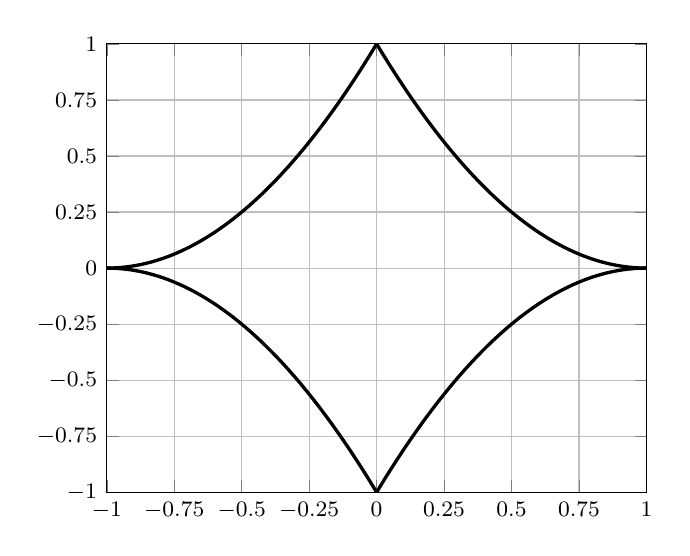
\begin{tikzpicture}
\begin{axis}[grid=major, xtick={-1,-0.75,...,1}, ytick={-1,-0.75,...,1}, xmin= -1, xmax=1, ymin=-1, ymax=1,tick label style={font=\footnotesize}]
\addplot[ very thick,samples=500] {(x-1)^2} ;
\addplot[ very thick,samples=500] {(-x-1)^2} ;
\addplot[ very thick,samples=500] {-(x-1)^2} ;
\addplot[ very thick,samples=500] {-(-x-1)^2} ;
\end{axis}
\end{tikzpicture}
\end{center}
\par
We can use the three points $(0,1), (1,0),(\frac{1}{2},\frac{1}{4})$ to determine the equation of the quadratic function in the top right corner.
The equation is $y = x^2-2x+1$, which if we integrate, we get $\frac{x^3}{3}-x^2+x+C$ and when evaluated from 0 to 1, we get $\frac{1}{3}$ as the area under the curve. However, since this is only the top right quadrant, we can leverage the x,y symmetry of the graph and multiply by 4 to find the total area. Thus the total area of the shape is $\frac{4}{3}$
  \item Use change of variables to derive a closed-form expression for the function
 \begin{align}
f(t) := \int_{0}^{t} \frac{x}{1+x^2} \diff{x}.
 \end{align}
\end{enumerate}
\subitem
So to solve this we're going to use u-substitution. Let $u= (1+x^2)$ and take the derivative of each side:
\begin{equation}
\begin{split}
   u = 1+x^2 \\
   du = 2xdx
\end{split}
\end{equation}

To solve the equation, start by substituting $u$ in for $1+x^2$, then substitute $\frac{\diff(u)}{2}$ for $x\diff{x}$, then integrate and sub $(1+x^2)$ for $u$
\begin{equation} \begin{split}
    f(t) := \int_{0}^{t} \frac{x}{u} \diff{x} \\
    \int_{0}^{t} \frac{1}{2} \frac{1}{u} \diff{u} \\
    \frac{\ln(u)}{2} + c \\
    \frac{\ln(1+x^2)}{2}+c
\end{split}
\end{equation}

  
\end{enumerate}
\break
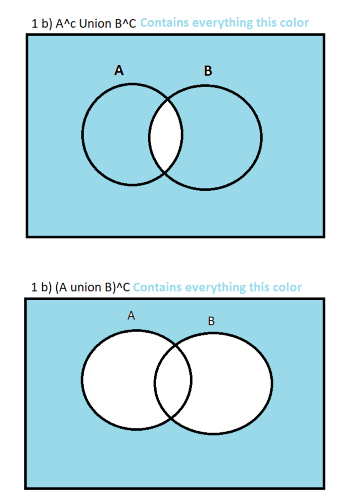
\includegraphics{hw01b.png} 
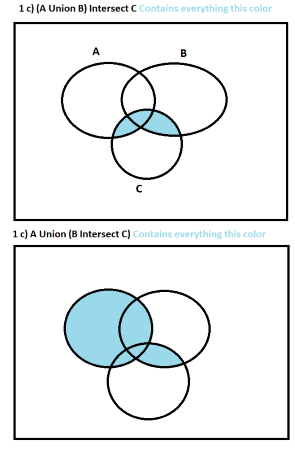
\includegraphics{hw01c.png} \\
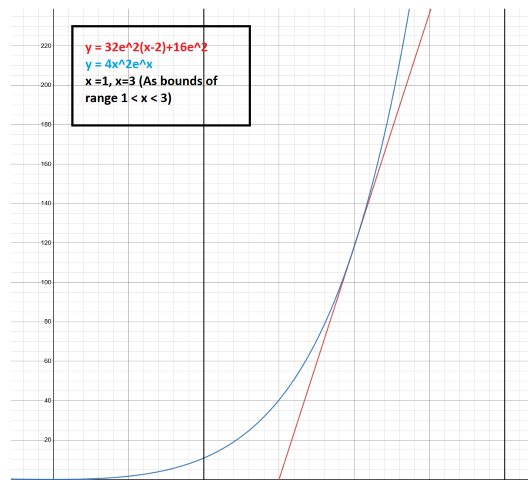
\includegraphics{hw03d.png}
\end{document}
